\section{Related Work and Motivation}
\label{sec:motivation}

\para{Related work}: 
Some SDN/SDC datapaths are recently proposed to offload complex,
stateful operations on packets (\eg, counting, flow security inspection and
congestion control) from the control plane (\eg, a base station) to data plane
devices (\eg, mobile devices) to improve the performance of SDN
applications~\cite{arashloo2016snap, heorhiadi2016simplifying, soule2014merlin,
benet2018mp, katta2016hula, gember2012stratos, anwer2015programming,
monsanto2012compiler,
kohler2018p4cep, bianchi2014openstate, opensdc} under dynamic
tactical environments. 
In these designs, results of offloaded operations are
stored by each data plane device independently. We refer to them as
\textit{local states}.
SOL~\cite{heorhiadi2016simplifying} and Merlin~\cite{soule2014merlin}
tackle the placement and configuration of data plane devices by solving
constrained path computation problems.
  P4CEP~\cite{kohler2018p4cep} and OpenSDC~\cite{opensdc} focus on expanding the
capability of data plane devices from packet processing to event processing.
SNAP~\cite{arashloo2016snap} designs a high-level programming system that
translates a high-level program to the configuration of
stateful operations in data plane devices. Despite these substantial efforts
on stateful SDC datapath, one major, common limitation of these systems is that the local states of each data plane device are not
shared with others. As we will show shortly in the motivating example, this would lead to
substantial resource under-utilization in SDC networks, impairing the
performance of SDC applications. 

To allow local state sharing between data plane devices, DDP~\cite{ddp} designs
some  primitives for distributed datapath update. Hula~\cite{katta2016hula} and
MP-HULA~\cite{benet2018mp} also design probing mechanisms for data plane devices
running load balancing applications to update their local states.  However,
manually configuring such low-level primitives on an application-by-application
basis is time-consuming and error-prone.


%There are some related work (\eg, \cite{arashloo2016snap},
%\cite{heorhiadi2016simplifying}, \cite{soule2014merlin}, \cite{benet2018mp},
%\cite{katta2016hula}, \cite{gember2012stratos}, \cite{anwer2015programming},
%\cite{hinrichs2009practical}, \cite{monsanto2012compiler},
%\cite{kohler2018p4cep}, \cite{mcclurg2016event}) for the offloading problem.




%But it does not consider sharing local
%state among switches. 



\begin{figure}[!htbp]
%\vspace{-2mm}
\centering
\begin{subfigure}{0.8\linewidth}
      \centering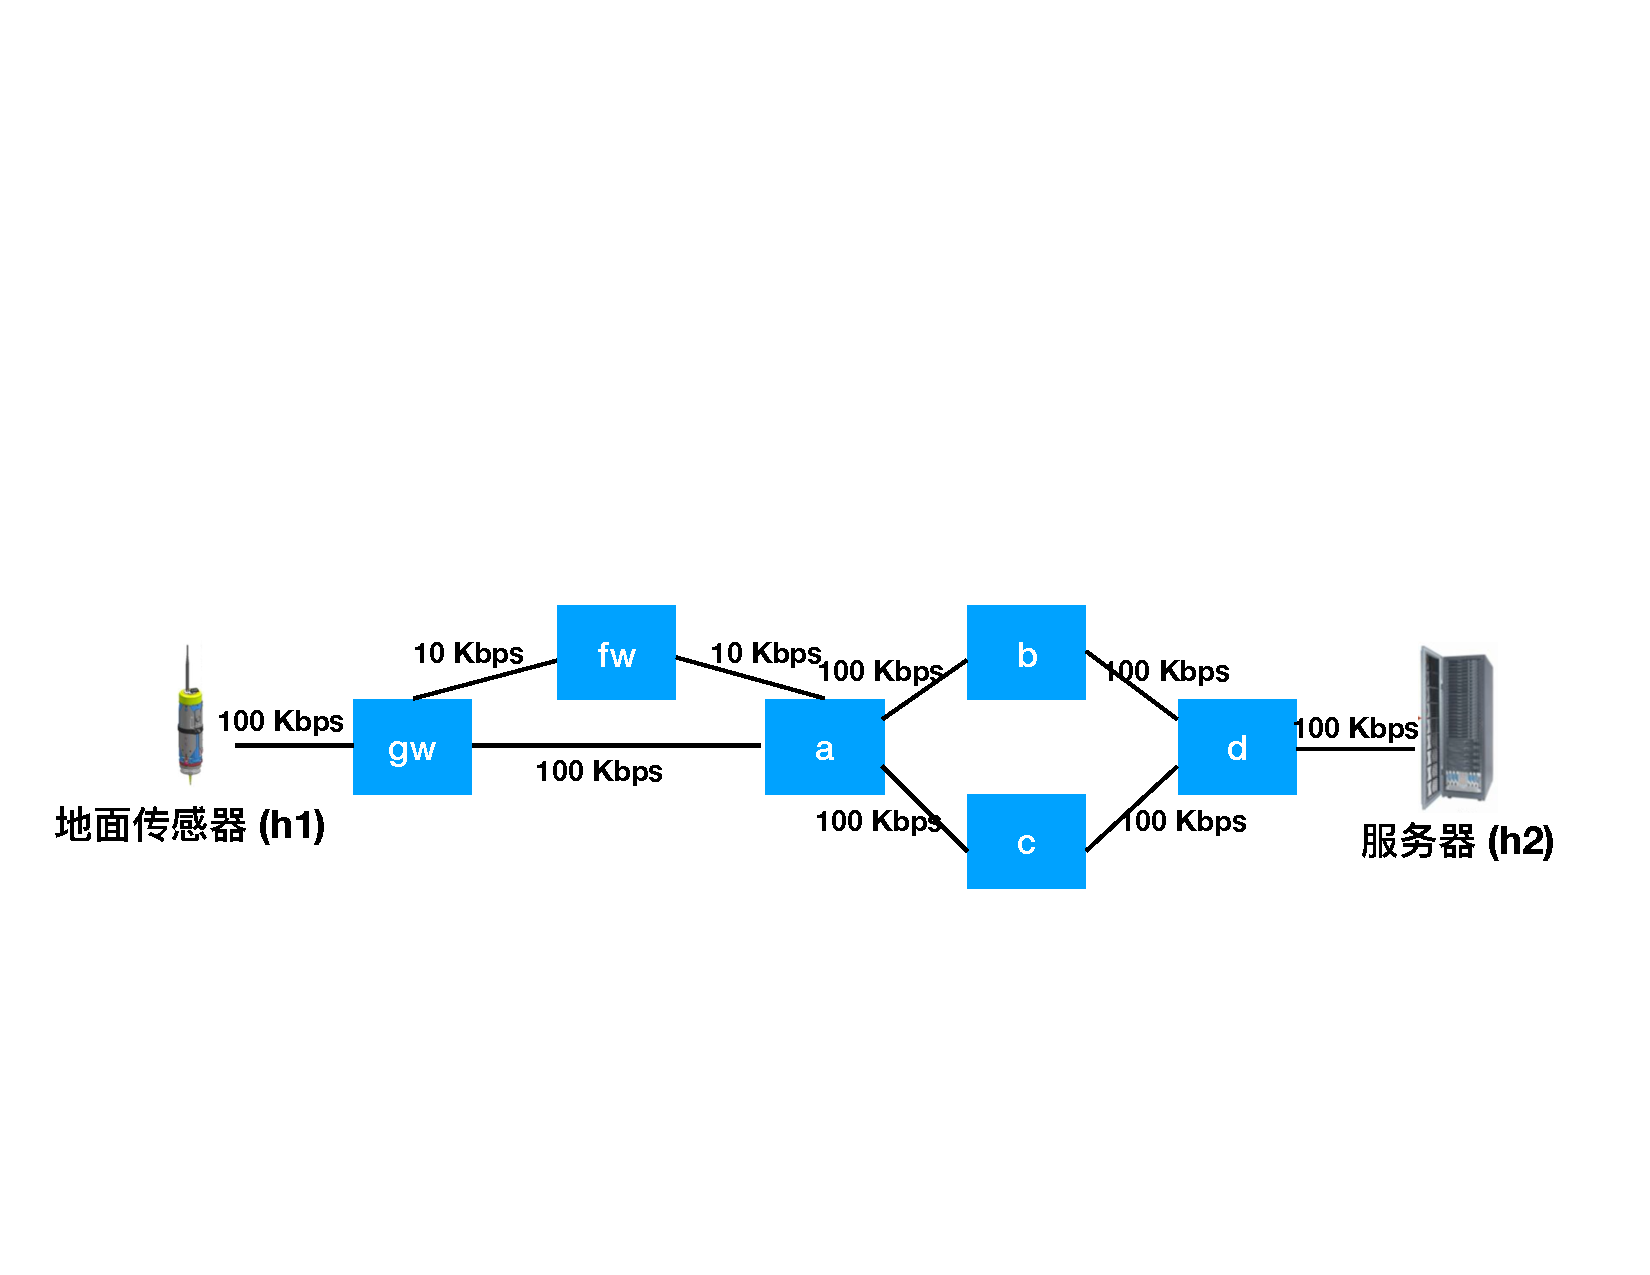
\includegraphics[width=\linewidth]{figures/ss-122.pdf}
      \caption{\label{fig:fw-topo} \small The network topology.}
\end{subfigure}
\hspace{0.03\linewidth}
\begin{subfigure}{0.8\linewidth}
      \centering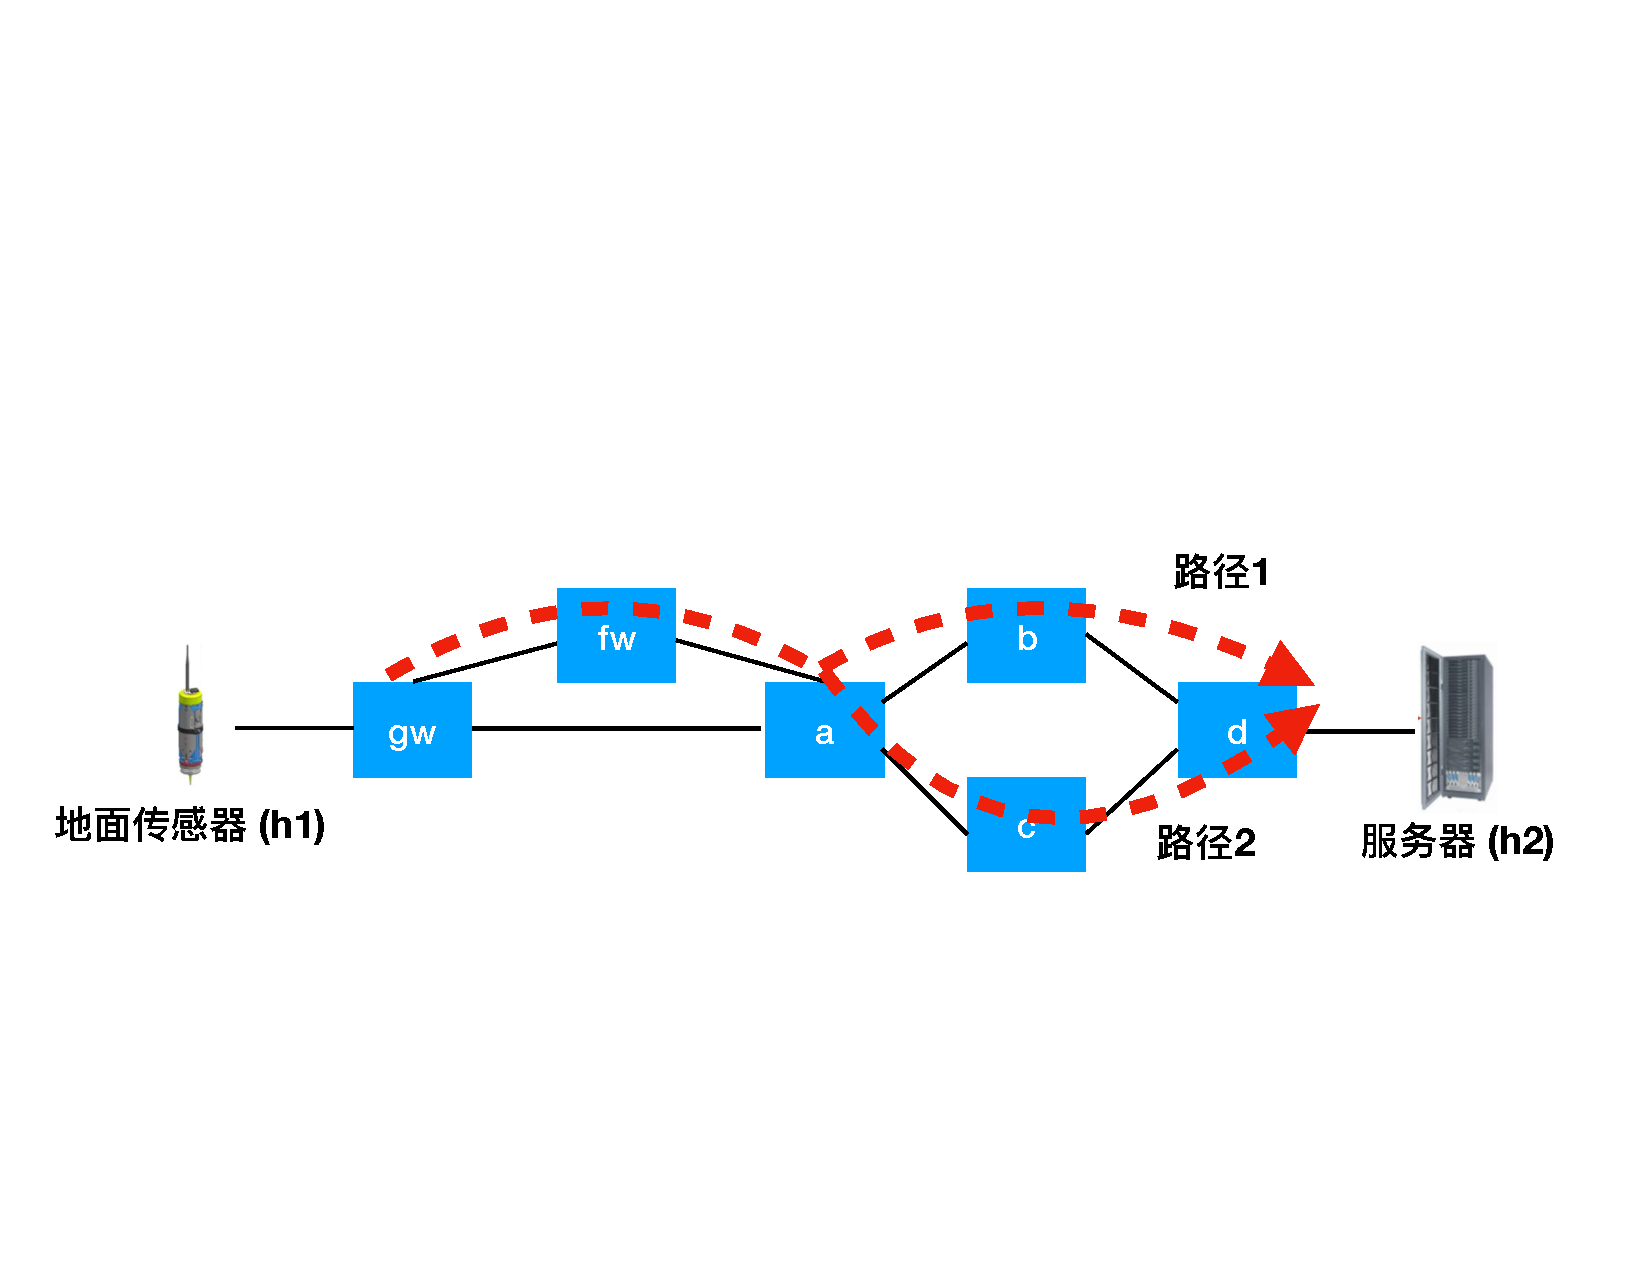
\includegraphics[width=\linewidth]{figures/ss-123.pdf}
      \caption{\label{fig:existing-result} \small The data plane configuration
	without local state sharing.}
\end{subfigure}
%\begin{subfigure}{0.8\linewidth}
%      \centering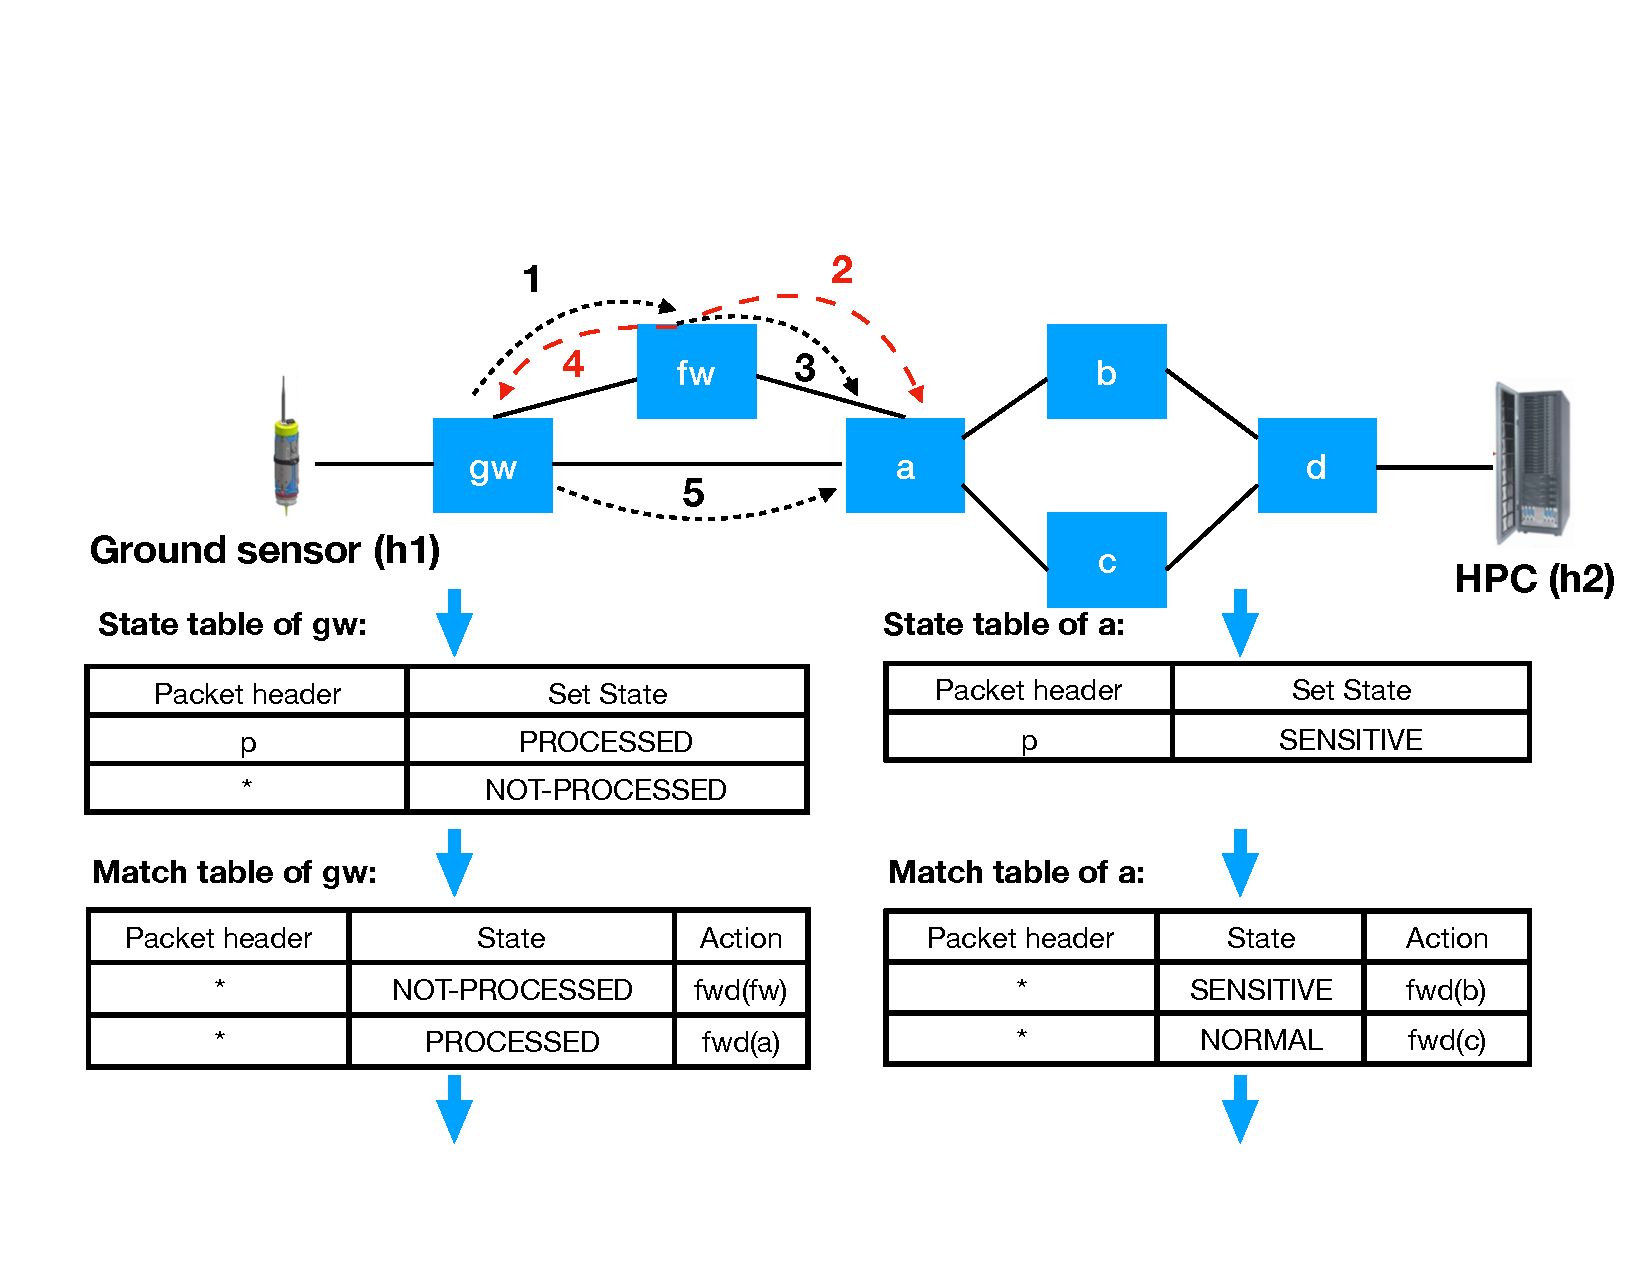
\includegraphics[width=\linewidth]{figures/ss-124.pdf}
%      \caption{\label{fig:dsdc-result} \small Configuration with \concept{}.}
%\end{subfigure}
%\vspace{-2mm}
%\caption{\footnotesize{The CDF of job latency local and remote jobs.}}
\caption{\small Motivating example: a data collection SDC application in a
	network with firewall.}
%\vspace{-2mm}
\label{fig:fw-example}
\end{figure}

\para{Motivation}: 
%We will motivate the \concept{} with a firewall example (as a
%running example in this paper) as shown in Fig.~\ref{fig:fw-topo}. 
We give an example to demonstrate the limitation of existing systems, and the
benefit of local state sharing. In particular, we consider a tactical network in
Fig.~\ref{fig:fw-example}(a), which consists of a ground sensor ($h_1$), a
middebox firewall ($fw$), a computing server ($h_2$), a gateway switch $gw$, and
other forwarding switches ($a$-$d$). The bandwidth of links $gw\rightarrow fw$,
and $fw \rightarrow a$ is
10 Kbps, while the bandwidth of all other links is 100 Kbps. 
The data collected by the sensor $h_1$
should first be sent to the firewall $fw$, which identifies whether the data
is sensitive or not based on the 5-tuple of
the packet carrying the data (\ie, srcAddr, dstAddr, srcPort, dstPort and
protocol). An SDC data collection application is running to send data collected
from the sensor to the server. The network operator wants to enforce the following policy: For any
data sent from $h_1$ to $h_2$, if it is sensitive, the
data should be forwarded along a route passing switch $b$, otherwise passing switch $c$. 

To enforce such a policy, state-of-the-art stateful datapath systems (\eg,
SNAP~\cite{arashloo2016snap}), which do not support local state sharing between
data plane devices, would compute the configuration as shown in
Fig.~\ref{fig:fw-example}(b).  Specifically, the gateway switch $gw$ forwards
all packets to the firewall $fw$. $fw$ identifies if it is sensitive or not, and
appends a tag on each packet to indicate the identification result before
sending to switch $a$. Switch $a$ then matches the tag of each arrival packet
and forwards them to $b$ (path1) or $c$ (path2) based on the matching result.

Though this configuration is correct, it does not fully utilize the resources in
SDC network, impairing the performance of the data collection application. Once
the sensitivity of a data flow is identified by the firewall $fw$, no future
packet of this flow needs to pass $fw$ again. Instead, they can be forwarded along path $gw, a, c, d $, or $gw, a, b, d$ with a higher transmission bandwidth. However, such a new
forwarding configuration cannot be realized without local state sharing between
the firewall $fw$, the gateway $gw$ and the switch $a$.

The above example demonstrates the benefits of local state sharing between data
plane devices in SDC. However, manually setting up the low-level configuration
for local state sharing is too time-consuming and error-prone. As such, we
design \concept, a novel SDC programming system to automatically translate
high-level SDC programs into datapath configurations with local state
sharing.

%for a higher throughput, without the need
%of passing the firewall again.
% by the
%firewall. The result gives correct paths for packets from $h_1$ to $h_2$ based
%on the firewall program. 


%Related with the local state sharing, MP-HULA~\cite{benet2018mp} and Hula~\cite{katta2016hula} use the probe packets to update the state variables for load-balancing which are the motivating examples of \concept{} but they do not consider the complex dependencies of middleboxes. 

%And for stateful SDN programming models, NetKAT~\cite{anderson2014netkat} defines a network querying language which is also different with \concept{} whose setting is to update state variables while keep packets processing. NetEgg~\cite{yuan2014netegg} proposes to use examples to specify the network stateful operations by keeping states in the controller while \concept{} targets to utilize state variables in stateful switches.




%
%In this section, we will motivate the general network-wide stateful packet processing with a load-balancing example as shown in Figure 1 (a). The example of load-balancing consists of $n$ clients and two servers. Clients try to establish connections to servers. For each connection, the destination can be either $server_1$ or $server_2$, while for the server side, it wants to balance the number of connections between the two servers. (Note that each connection can establish multiple connections to servers.)
%
%%Figure 1 LB example
%\begin{figure}[!htbp]
%%\vspace{-2mm}
%\centering
%\begin{subfigure}{0.47\linewidth}
%      \centering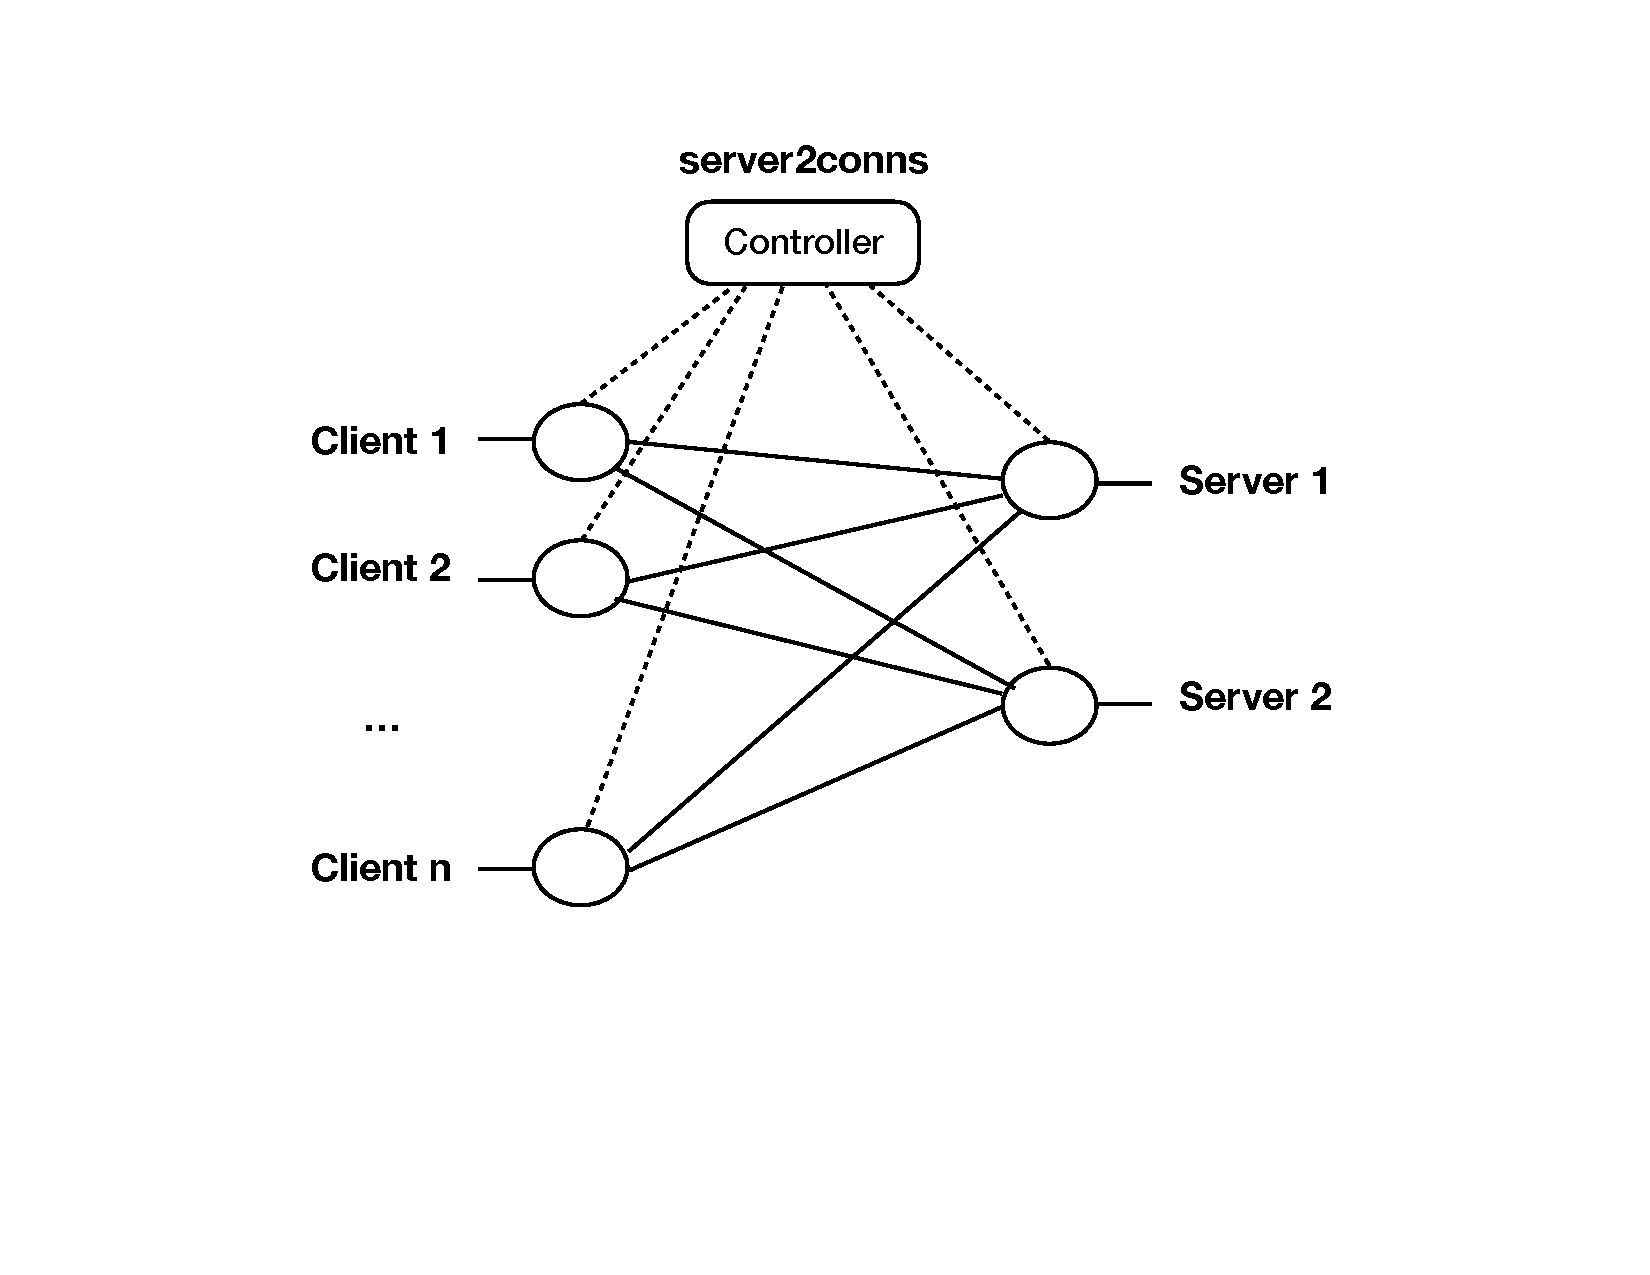
\includegraphics[width=\linewidth]{figures/65.pdf}
%      \caption{\label{fig:lb-example} \small A simple SDN design.}
%\end{subfigure}
%\hspace{0.03\linewidth}
%\begin{subfigure}{0.47\linewidth}
%      \centering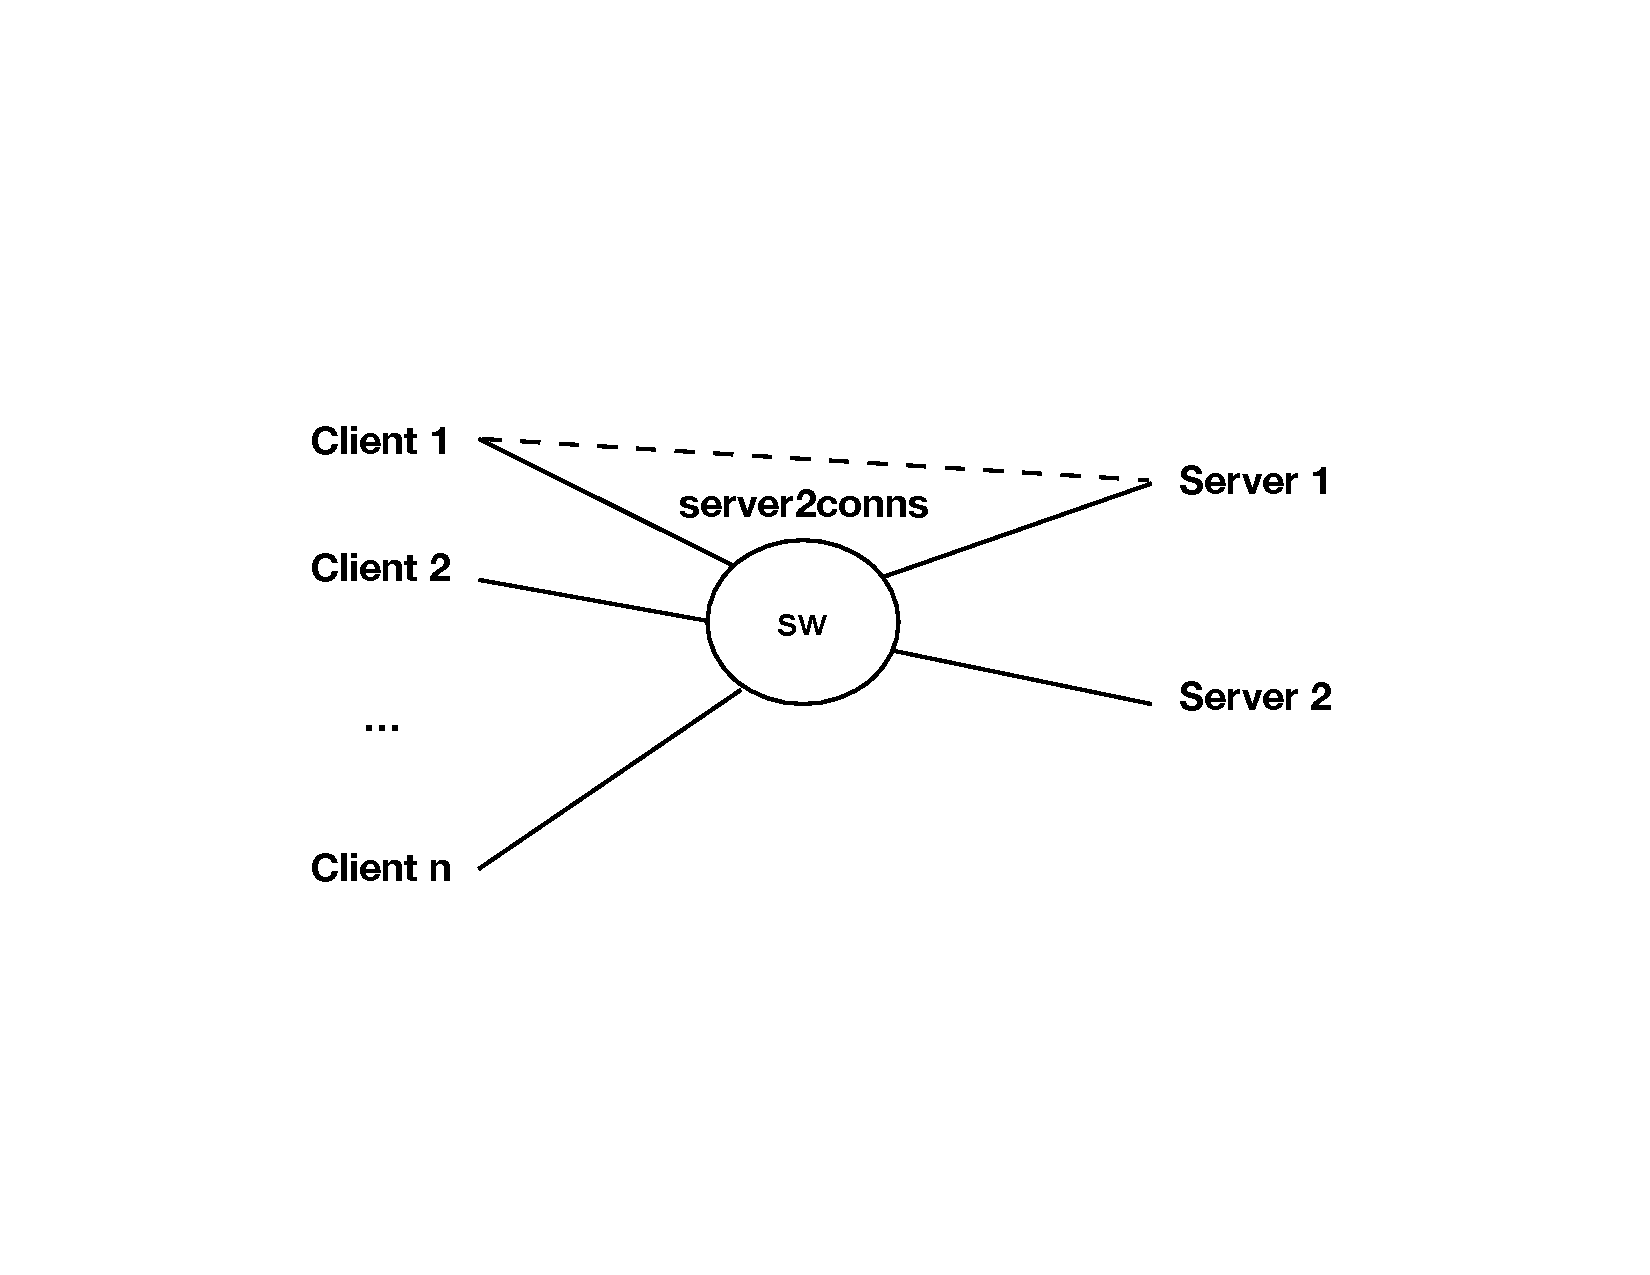
\includegraphics[width=\linewidth]{figures/66.pdf}
%      \caption{\label{fig:fm-example} \small Stateful switch design.}
%\end{subfigure}
%\begin{subfigure}{0.47\linewidth}
%      \centering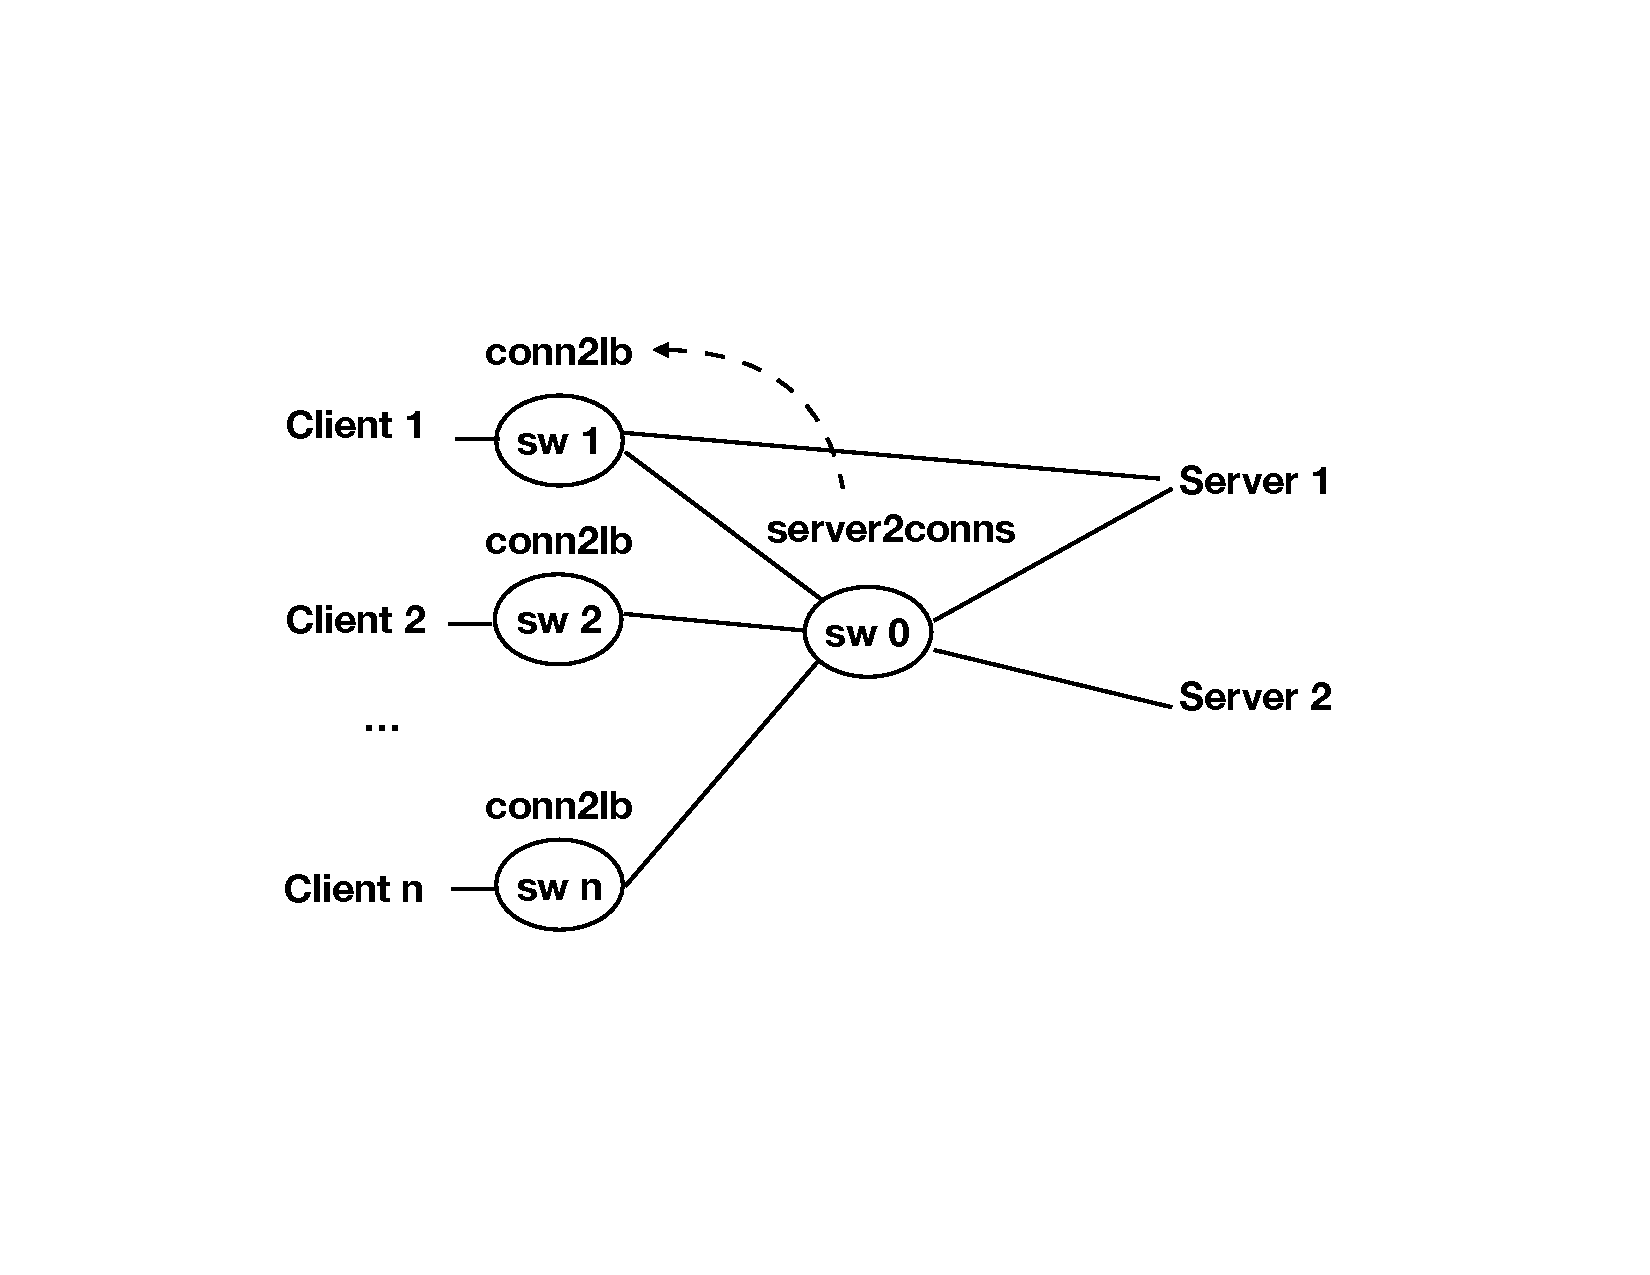
\includegraphics[width=\linewidth]{figures/67.pdf}
%      \caption{\label{fig:fm-example} \small Two-state design.}
%\end{subfigure}
%%\vspace{-2mm}
%%\caption{\footnotesize{The CDF of job latency local and remote jobs.}}
%\caption{\small Examples of load-balancing.}
%%\vspace{-2mm}
%\label{fig:mtv-example}
%\end{figure}
%
%For a simple SDN design, the load-balancing can be done at the controller which keeps a map (denoted as \emph{server2conns}) whose key is a server id and the value is the number of connections currently established for the server. Then, when a client needs to start a new connection, the first packet of the connection will be forwarded to the controller where a server is assigned to the connection based on the map in the controller. The shortage of this design is the latency added for the connection between switches and the controller. By leveraging the stateful switches ([XXX]), the state (\ie, \emph{server2conns}) can be offloaded to the switches where the packets can read states without involving the controller.
%
%A stateful switch design where the load-balancing can be done in the data planes is shown in Figure 1 (b). To achieve the load-balancing in the data planes, the state \emph{server2conns} is kept in the stateful switch $sw$. When a client needs to start a new connection, the first packet will be forwarded to $sw$ where a server will be assigned to the packet (also the state \emph{server2conns} is updated). Then, the packet will be forwarded to the assigned server without involving the controller. The stateful switch design removes the latency between the controller and switches but the paths between clients and servers have a constraint that they must pass through $sw$ even the server has been assigned. (Though the dot line in Figure 1 (b) is the optimal path between $client_1$ and $server_1$, it cannot be used.) This is because \emph{server2conns} is a global variable for all the connections; it cannot be distributed among multiple switches.
%
%To make optimal path available in the stateful switch design, one solution is to change the path after the processing of load-balancing in $sw$(\ie, processing of \emph{server2conns}). To achieve the changing of paths, other state variables are required. As shown in Figure 1 (c), $sw_0$ keeps the state \emph{server2conns} and other stateful switches $sw_1$, $sw_2$, ... $sw_n$ (we assume $client_i$ connects to $sw_i$) keep the states \emph{conn2lb} (each switch maintains \emph{conn2lb}) where the key is the connection and the value is the status of load-balancing (\ie, to indicate whether the load-balancing has been processed for the connection). Consider $client_1$ starts a new connection, the first packet will arrive at $sw_1$. Based on \emph{conn2lb}, if the status of the connection indicates the server is not assigned, then the packet will be forwarded to $sw_0$. After the processing in $sw_0$, it updates the state \emph{conn2lb} in $sw_1$ to set the value to indicate the load-balancing is done. Then, based on \emph{conn2lb} in $sw_1$, all the following packets from $client_1$ to the server can use the optimal path which may not pass through $sw_0$.
%
%Though the two-state design resolves the issues of other designs (\ie, additional latency and not optimal path), this cannot be implemented with existing work. The most relevant work, SNAP [XXX], achieves a network-wide stateful packet processing, but the data dependency between \emph{conn2lb} and \emph{server2conns} (\ie, packet reads \emph{conn2lb}; packet reads \emph{server2conns}; packet writes \emph{conn2lb}) makes the two state variables must be assigned in a single stateful switch, which cannot achieve the optimal path requirement. Therefore, in this paper, we propose the general network-wide stateful packet processing which provides a high flexibility for the state updates of stateful packet processing.






